\phantomsection

\section*{Удиртгал}
%Системтэй холбоотой танилцуулгыг энэ хэсэгт бичнэ.
\subsection*{Зорилго}
\par Энэхүү системийн зорилго нь хэрэглэгчийн  өдөр тутмын хувцаслалтад зарцуулах цаг хугацааг хэмнэж хэрэглэгчийн өөртөө итгэх итгэлийг нь нэмэгдүүлэх юм. Өөрөөр хэлбэл өөрт байгаа хувцсаа зар мэдээ, профайл хэсэгт оруулан thrift shop буюу цөөн тоогоор өмссөн хувцсаа бусдад хандивлах, өөрөөр хувийн стилисттэй холбогдон хувийн өнгөний зохицол, загвараа тодорхойлуулах гэх мэт байгалийн уур амьсгалд ч эергээр нөлөөлөхөөр маш өргөн, нээлттэй, уян хатан систем бий болгохыг зорьж байна.
\subsection*{Зорилт}
\begin{enumerate}
   \item Бодит веб систем аппликейшн хөгжүүлэх 
   \item Хэрэглэгчийн хувцсыг зөв катигорчлон ангилах
   \item Бүтээгдэхүүний каталогийг хэрэглэгчдэд зөв, ойлгомжтой харуулах
   \item AI ашиглан хэрэглэгчид шинэ look санал болгох
   \itemАлгоритмуудыг тасралтгүй сайжруулан, судлах
\end{enumerate}
\subsection*{Систем хөгжүүлэх үндэслэл}
\paragraph{}Дэлхий даяар хиймэл оюун дээр суурилсан технологиуд хурдацтай хөгжиж байгаа билээ. Үүнийгээ дагаад бүхий л салбаруудад энэхүү  технологийг  ашиглан хэрэглэгчийн өдөр тутмын амьдралд оновчтой зөв шийдвэл гаргах, цаг хугацаа хэмнэх, эрүүл  бөгөөд аз жаргалтай амьдрахад маш их туслалцаа үзүүлдэг. Харин бидний хөгжүүлж буй “Recommendation clothes” нь дээр дурдсан хиймэл оюун ухааныг ашиглан хэрэглэгчид хэрэгцээтэй хувцаслалтыг хүргэдэг систем юм.\\
Энэхүү системийг хөгжүүлэх үндэслэл нь:


\par Монгол улс нь   эрс тэс уур амьсгалтай учир үүнд таруулан оновчтой хувцаслахад хялбар байдаггүй. Бидний хийсэн судалгаанаас үзэхэд Монголд амьдарч буй хүмүүсийн дийлэнх хувь нь зохистой хувцаслах тал дээр тодорхой хэмжээний асуудалтай байдаг нь ажиглагдсан.
\begin{figure}[H]
    \centering
    \caption{Хувцаслалтаа тохируулахад хэр хүндрэлтэй санагдаг вэ? \cite{grap1}}
    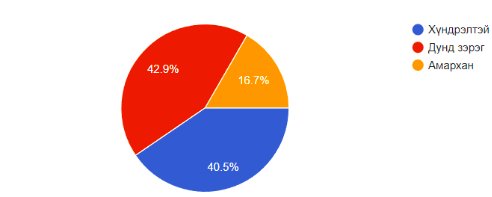
\includegraphics[width=\textwidth]{figures/Screenshot 2024-10-03 at 15.59.07.png}
    
    \label{fig:sudalgaa1}
\end{figure}
\begin{figure}[H]
    \centering
    \caption{Маргааш юу өмсөх вэ? гэж бодож байсан уу? \cite{grap2}}
    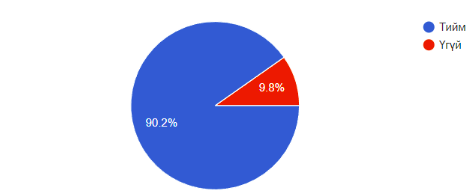
\includegraphics[width=\textwidth]{figures/Screenshot 2024-10-03 at 16.17.44.png}
    
    \label{fig:sudalgaa}
\end{figure}
\begin{figure}[H]
    \centering
    \caption{Цаг агаарын өөрчлөлтөөс болоод тохиромжгүй хувцалж байсан уу? \cite{grap3}}
    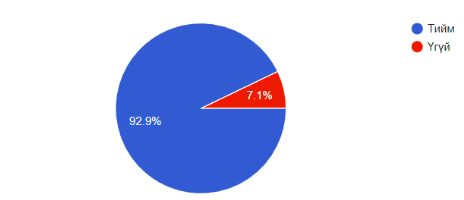
\includegraphics[width=\textwidth]{figures/Screenshot 2024-10-03 at 17.19.53.png}
    
    \label{fig:sudalgaa}
\end{figure}



\subsubsection*{Судалгаа}
\parДээрх судалгаанаас авч үзэхэд хувцас сонголт хийх нь Монголд амьдарч буй хүмүүст тодорхой хэмжээгээр хүндрэл үүсдэг бөгөөд энэ асуудалд хүн болгон оновчтой шийдвэр гаргаж чаддаггүй гэдгийг харуулж байна.Энэ нь жижиг асуудал хэдий ч хүн бүрийн амьдралд тулгардаг асуудал юм.Уг асуудлыг манай систем шийдсэнээр тодорхой хэмжээгээр асуудлыг багасгаж хувь хүний өөртөө итгэлтэй байдал болон сэтгэл ханамжийг өгч тухайн хэрэглэгчийн өдрийн бүтээмжийг нэмэгдүүлнэ.

\subsubsection*{Байгаль эх дэлхий} - Хүн төрөлхтөн өдгөө жил бүр 2.12 тэрбум тонн хог хаягдал бий болгож буй. Тэдгээрийг ачааны машинд овоолон цуваа үүсгэх юм бол дэлхийг 24 удаа ороож хүрэхүйц их хэмжээтэй байдаг. Үүний 2\% орчим нь хаягдал хувцас байдаг бөгөөд энэхүү хог хаягдлын дөнгөж 20 хувийг нь дахин боловсруулж хэрэглэгддэг үлдсэн 80 хувь байгальд хаягдаж бохирдол үүсгэдэг. Магадгүй бид 20-ос илүү хувийг дахин боловсруулах , байгальд хаягдаж байгаа хувцасны тоог багасгах зорилгоор системийг цааш хөгжүүлэн хэрэглэгчид  цөөн тоогоор өмссөн хувцсаа бусдад хандивлах эсвэл бүтээлч байдлаар хэрхэн нөхөн сэргээж хэрэглэх талаар санал болгоно. 
\subsubsection*{Цахим худалдаа}Дижитал платформ хөгжиж буй өнөө үед онлайн дэлгүүрүүд эсвэл загварын компаниуд хиймэл оюун ухаанд суурилсан зөвлөмжийн системийг нэвтрүүлэх боломжтой. Эдгээр системүүд нь хэрэглэгчдийн сонголт, хэрэгцээнд нийцүүлэн хувцасны хэв маяг, биеийн хэлбэр, соёлын онцлог зэрэг хүчин зүйлс дээр тулгуурлан хувь хүнд хувцаслалтын төрлөөр зөвлөмж өгөх юм.

\subsubsection*{Системийн холбоо}Манай систем сүлжээ дэлгүүрүүдтэй хамтран ажиллаж хэрэглэгчдэд хэрэгцээтэй бараа бүтээгдэхүүнийг санал болгон онлайн худалдааны орчныг бий болгож хэрэглэгчийн өөрт тохирсон хувцсыг хайдаг байсан цаг хугацааг хэмнэнэ.

\subsection*{Судлагдсан байдал}
% Энд сонгосон сэдэвтэй холбоотой хийгдсэн ажил, судалгааны талаар товч дурдана. Бүлэг нэгт ижил төстэй системийн судалгаа гэдэг хэсэгт илүү дэлгэрэнгүй мэдээллийг бичнэ.
\par Манай багийн судалж буй сэдвийн хүрээнд ( Recommendation clothes ) гадаад болон дотоодын зах зээлд:
\par \textbf{Дотоодын зах зээлд}:  Судалгаагаар Монгол улсад хиймэл оюун, машин сургалт зэрэгт технологиуд дээр суурилсан хувцас санал болгох систем, веб, апп байдаггүй бөгөөд энэхүү технологийг ашиглан хөгжүүлснээр манай систем монголдоо анхдагч нь болох юм. 
\par \textbf{Гадаадын зах зээлд}: Хэрэглэгчийн хувийн сонголт, хэв маяг, биеийн хэлбэр, төсөвт санхүүд тань тохирсон хувцасны зөвлөмжийг өгөх зорилготой хэд хэдэн томоохон системүүд байдаг байна. Тэдгээр нь ихэвчлэн хэрэглэгчээс загварын асуулт хариулт авах, худалдан авалтын түүх, санал хүсэлт зэрэг янз бүрийн мэдээллүүд дээр тулгуурлан зөвлөгөө өгөх мөн таны загварын чиг хандлагыг тань бий болгоход, туслах зориулалттай.
\par \textbf{Stitch Fix:}
\begin{figure}[!http]
	
\includegraphics[scale=1]{figures/download.png}
\end{figure}
\par Stitch Fix бол хиймэл оюун ухаан ашиглан үйлчлүүлэгчдэдээ хувцас санал болгох зорилготой онлайн хувийн загварчлалын үйлчилгээ юм. Хэрэглэгчид загварын чиг хандлагынхаа талаар асуумжийг бөглөх, мөн сайтаас худалдан авсан зүйлсийнхээ талаар санал хүсэлтээ өгдөг бөгөөд энэ нь тань дээр гарж ирэх, санал болгох зөвлөмж хувцаслалтуудыг сайжруулахад ашиглагдана. Stitch Fix-ийн зөвлөмжийн систем нь хэрэглэгчийн сонголт, биеийн хэмжээ, хэв маягт тань дүн шинжилгээ хийж, загварыг тань тодорхойлоход тусална.
\par \textbf{ASOS(AsSeenOnScreen):}
\begin{figure}[!http]
	
\includegraphics[scale=0.8]{figures/images.png}
\end{figure}
\par Энэхүү систем нь мөн адил таны сонирхол болоод одоогийн тренд болоод буй загварын чиг хандлаг дээр тулгуурлан хувцаслалтыг тань сонгоход тусална.
Өөрийн сонирхсон хувцсан дээр даран(хайж сонгон) орсны дараа сонгосон хувцасны модель өмссөн олон талын зураг, үнийн мэдээлэл, өнгө, хэмжээ, сагсанд хийх, хадгалах, түүнтэй адил төстэй хувцас түүний үнэ болон тэрхүү хувцсан дээр зохицох хувцсыг(цамц гутал гэх мэт) харуулна.
\subsection*{Шинэлэг тал}
\begin{enumerate}
   \item \textbf{Thrift shop болон хувцасны зар сурталчилгаа:} Хэрэглэгчид өөрийн хэрэглэж байсан, цөөн өмссөн хувцсыг зар сурталчилгааны хэсэгт оруулж бусдад хямд үнээр худалдаалах эсвэл хандивлах боломжтой. Энэ нь хувцас хаягдал багасгахад хувь нэмэр оруулж, хэрэглэгчдэд шинэ орлого олох боломжийг олгоно.
   \item \textbf{Хувийн стилист үйлчилгээ:} Хэрэглэгч өөрийн хувийн стилисттэй холбогдож, өнгөний зохицол, хувцасны стиль болон загварын зөвлөгөө авах боломжтой. Энэ нь хувцаслалтад итгэлтэй байх, загварлаг харагдах, хувь хүний онцлогийг тодруулахад тусалдаг.
   \item \textbf{Байгальд ээлтэй шийдэл:} Хувцас хандивлах болон дахин ашиглах нь байгаль орчинд эергээр нөлөөлөх бөгөөд хувцас хаягдлыг бууруулж, нөөц баялгийг хэмнэх ач холбогдолтой. Энэ нь хэрэглэгчид байгаль орчинд хариуцлагатай хандах боломжийг олгоно.
\end{enumerate}
\subsection*{Ач холбогдол}
%Энд зорилгод хүрэх зорилтуудыг бичнэ.
\begin{enumerate}
   \item \textbf{Цаг хугацаа хэмнэх:} Хувцас сонгох, зохицуулах, худалдаалах зэрэг үйл ажиллагаануудыг илүү хялбар болгосноор хэрэглэгчийн цаг хугацааг хэмнэнэ.
   \item \textbf{Өөртөө итгэх итгэлийг нэмэгдүүлэх:} Хувийн стилистээс авсан зөвлөгөө болон загварын хувьд итгэлтэй болох нь хэрэглэгчийн өөртөө итгэх итгэлийг нэмэгдүүлнэ.
   \item \textbf{Санхүүгийн хувьд ашигтай:} Хэрэглэгчид хуучин хувцсаа зарж, шинэ орлого олох боломжтой болохын зэрэгцээ чанартай, хямд хувцас авах боломжтой.
   \item \textbf{Эко сэтгэлгээтэй нийгэмд хувь нэмэр оруулах:} Байгальд ээлтэй хэрэглээг дэмжих замаар байгаль орчны асуудалд анхаарал хандуулсан хариуцлагатай хэрэглэгчдийг бий болгох.
\end{enumerate}
%Хөгжүүлэх гэж буй системийн ач холбогдолтой талуудыг тоочиж бичнэ.
Энэ систем нь нийгэмд эерэг өөрчлөлт хийх, байгаль орчныг хамгаалахад хувь нэмэр оруулах шинэлэг бөгөөд олон талт шийдэл болно.

\subsection*{Системийн хүрээ хязгаар}
%Хөгжүүлэх гэж буй системийн хамрах хүрээг нарийн тодорхойлж энд заана.
Манай төслийн хамрах хүрээн манай улсаас гадна гадны орнуудад ч бас хэрэглэж болно. Манай төсөл нь тухайн байрштлын цаг агаар болон бусад хүчин зүйлүүдийг тооцолон хамгийн тохиромжтой бөгөөд тааламжит хуцасыг сонгож өгнө.


